\documentclass[11pt,a4paper]{article}

\usepackage[margin=2.2cm]{geometry}
\usepackage[T1]{fontenc}
\usepackage{lmodern}
\usepackage{amsmath,amssymb}
\usepackage{graphicx}
\usepackage{booktabs}
\usepackage{tabularx}
\usepackage{array}
\usepackage{float}
\usepackage{needspace}
\usepackage{caption}
\usepackage{enumitem}
\usepackage{xcolor}
\usepackage{algorithm}
\usepackage{algpseudocode}
\usepackage[hidelinks]{hyperref}

\graphicspath{{figures/}}
\setlist{itemsep=2pt,topsep=4pt}
\captionsetup{font=small,labelfont=bf}
\newcommand{\ours}[1]{\textcolor[HTML]{1B7F5A}{#1}}

\newcommand{\fppvsMinAcc}{76.6}
\newcommand{\fppvsMaxAcc}{91.0}
\newcommand{\fppvsMeanAcc}{83.7}
\newcommand{\fppvsWorstScenario}{Metro 1.1}
\newcommand{\fppvsLowestRun}{73.5}
\newcommand{\trainSeconds}{60}
\newcommand{\numSeeds}{5}
\newcommand{\origMinAcc}{65.6}
\newcommand{\origMaxAcc}{77.0}
\newcommand{\origMeanAcc}{71.1}
\newcommand{\origGainMin}{11.0}
\newcommand{\origGainMax}{14.0}
\newcommand{\origGainMean}{12.6}
\newcommand{\zhangMinAcc}{43.0}
\newcommand{\zhangMaxAcc}{53.1}
\newcommand{\zhangMeanAcc}{48.0}
\newcommand{\zhangGainMean}{35.7}

\title{\textbf{Fairness-aware and Parallelized SFC Placement with VNF Sharing:\\
Implementation, Limitations and Modifications}\\[4pt]
\large Advanced Computer Networks: Project Report}
\author{23CSB0B03 \quad 23CSB0B17 \quad 23CSB0B23 \quad 23CSB0B56}
\date{}

\begin{document}
\maketitle

\begin{abstract}
In this project we looked at FPPVS, a framework by Zhu, Li and
Rezaeipanah~\cite{fppvs}. It places service function chains (SFCs) in
MEC-enabled IoT networks, and it does this using SFC parallelization, VNF
sharing, fairness-aware allocation and federated deep reinforcement learning
(FDRL). We built a full Python implementation of it. Our first version was
honestly bad: it accepted only about 10\% of requests, which is even worse than
just placing things randomly. We traced this back to a few gaps, some in the way
the problem was specified and some in our own implementation, and then we
changed the formulation and the algorithm. The changes are: Poisson arrivals at
a stated offered load, a placement mask that checks compute, bandwidth and
latency before a data center is picked, a per-data-center actor network with a
placement prior, honest accounting for shared VNF instances, rollback-and-retry
admission, and fixed federated training. We tested on synthetic Backbone (24
nodes) and Metro (17 nodes) topologies at three heavy load levels (offered demand
at 90\%, 100\% and 110\% of network capacity). Here the updated FPPVS accepts
between \fppvsMinAcc\% and \fppvsMaxAcc\% of requests on a hold-out stream (mean
of \numSeeds{} seeds). Under the same conditions, the original FPPVS as written
in the paper accepts \origMinAcc--\origMaxAcc\%, a 2022 SFC-placement method by
Zhang et al.\ accepts \zhangMinAcc--\zhangMaxAcc\%, and greedy and random
placement stay between 49\% and 59\%. Coming to resources, updated FPPVS holds
about half the link bandwidth per running service compared to greedy and random,
11\% less than the original FPPVS, and kind of the same as the 2022 adaptation.
\end{abstract}

\noindent\textbf{How to read this report.} Whenever we talk about the original
paper, we call it ``the paper'' or ``the original work''. Anything our team
designed, changed or measured is marked as ours, and all of it is summarised in
Table~\ref{tab:contrib}.

%=====================================================================
\section{Introduction}
%=====================================================================

\subsection{Problem addressed}
Network Function Virtualization (NFV) takes dedicated middleboxes, like
firewalls (FW), intrusion detection (IDS), deep packet inspection (DPI), load
balancers (LB) and NAT, and replaces them with software Virtual Network
Functions (VNFs). A network service is just an ordered list of VNFs, and this
list is called a Service Function Chain (SFC). In a Mobile Edge Computing (MEC)
network, the VNFs run on small edge data centers (DCs) that don't have much
compute, and the DCs are connected by links that have limited bandwidth and some
latency. The \emph{SFC placement problem} asks this: for every request that
comes in, which DC should each VNF run on, and how should traffic be routed
between them, so that capacity, bandwidth and the request's latency limit are
all respected. The problem is NP-hard, and it has to be solved online, because
requests keep coming one after another and leave once their lifetime is over.

\subsection{Motivation}
In IoT/MEC settings, two things make this problem harder. First, if every packet
goes through every VNF one by one, the end-to-end latency keeps growing as the
chain gets longer. Second, a lot of requests fight for the same small edge DCs,
so a placement policy that only looks at the current request can starve the
later ones. Existing methods mostly handle only one of these at a time: network
function parallelism brings latency down, and VNF reuse brings resource use
down. Fairness between competing flows is usually just ignored.

\subsection{Main contributions of the original paper}
The paper~\cite{fppvs} proposes FPPVS, which puts together four ideas:
\begin{enumerate}
  \item \textbf{SFC parallelization (Algorithm 1).} VNFs are split into two
  kinds. \emph{Shapers} change packets and have to stay in order, and
  \emph{monitors} only read packets. Monitors are moved onto branches that run
  side by side with the main chain, and a dependency matrix says where each
  branch has to join back. So the sequential SFC (s-SFC) turns into a directed
  acyclic graph (p-SFC), and latency is measured on its critical path.
  \item \textbf{VNF sharing with demand prediction.} Before making a new VNF
  instance, the method first tries to reuse a live instance that fits. A
  bounded SFC queue network (SQN) and an LSTM predict the upcoming demand for
  each VNF type.
  \item \textbf{Fairness-aware allocation.} A concave $\alpha$-fair utility over
  flow throughput is part of the objective, so a few heavy flows can't grab all
  the resources. Jain's fairness index (JFI) is reported.
  \item \textbf{Federated actor-critic learning.} Local agents with a CNN
  actor-critic place the VNFs, and a cloud server combines their models using
  federated averaging (FedAvg)~\cite{fedavg}. For exploration, it uses a
  reward-driven adaptive $\epsilon$-greedy rule.
\end{enumerate}
The paper reports 88.1\% service acceptance on a backbone topology and 75.9\% on
a metropolitan topology, which is ahead of four baselines (RVNF, DRL-SFCP, PVFP
and DPC).

%=====================================================================
\section{Limitations of the Original Work}
%=====================================================================

Here are the limitations we ran into while implementing the paper. Some of them
are gaps in what the paper specifies, so it can't be reproduced exactly. Others
are design problems that only showed up once the method was actually running.
Table~\ref{tab:limits} says which ones our project deals with.

\begin{enumerate}[label=\textbf{L\arabic*.}]
  \item \textbf{The workload is under-specified.} The paper fixes a mean
  service lifetime of 1000 time units and 4000 requests, but it never gives
  the arrival rate. And the arrival rate is what decides how many SFCs are
  active at the same time, so it basically decides the acceptance ratio. When we
  used one arrival per time unit, about 1000 SFCs would need to be active at
  once, but a 24-node network with 10--20 compute units per DC can only hold
  about 70--100.
  \item \textbf{Datasets and code are not available.} The USAnet and Italian
  operator topologies, the traffic traces, the MATLAB code and the baseline
  configurations are not published. So results can only be compared in spirit.
  \item \textbf{Latency is checked too late, and only one hop ahead.} The paper
  prunes nodes that don't have enough compute or free bandwidth, and then picks
  the current node or a neighbour for the next VNF. The latency limit is checked
  only once the whole chain is placed, and the neighbour rule can walk the agent
  into a corner where no neighbour fits the next VNF. So an agent can spend a
  full episode building a placement that just gets rejected at the last step.
  \item \textbf{The sharing model can overbook capacity.} The paper doesn't say
  how much capacity a shared instance reserves, or when that capacity is let go.
  A natural reading, which our first version followed (instances sized at three
  times the demand, but only one times reserved), lets the pool use capacity that
  the DC doesn't actually have.
  \item \textbf{The CNN input is tied to one topology.} The paper joins all the
  features into one fixed-length vector for its CNN. Because of this, the network
  size depends on the number of DCs, its $3\times3$ convolutions mix up the
  features of DCs that just happen to sit next to each other in the vector, and
  nothing in the model reflects that the DCs are interchangeable. (Our first
  implementation made this even worse by adding global pooling, which lost track
  of which column belonged to which DC; see below.)
  \item \textbf{Each episode is one request.} The reward only sees the current
  request. Effects on later requests, like fragmentation or a full link, reach
  the agent only indirectly.
  \item \textbf{Resource efficiency is reported only as utilization.} Higher
  utilization can mean better packing, but it can also mean more waste per
  request. The paper doesn't report how much resource each served SFC holds over
  time.
\end{enumerate}

\begin{table}[H]
\centering\small
\caption{Limitations and how our project handles them.}
\label{tab:limits}
\begin{tabularx}{\linewidth}{l X l}
\toprule
 & Our treatment & Status \\
\midrule
L1 & Poisson arrivals whose rate is set from an explicit offered load $\rho$ & \ours{Addressed} \\
L2 & Synthetic graphs of the same size; simple, documented baselines & Partly (data still missing) \\
L3 & Look-ahead mask on compute, every routed link and the latency bound & \ours{Addressed} \\
L4 & Per-instance overhead model, all usage counted against physical capacity & \ours{Addressed} \\
L5 & Per-column actor with shared weights plus a learnable placement prior & \ours{Addressed} \\
L6 & Placement prior with future-hop term; rollback-and-retry admission & Partly \\
L7 & New metrics: resources held per running SFC and resource-time per accepted SFC & \ours{Addressed} \\
\bottomrule
\end{tabularx}
\end{table}

\paragraph{Problems in our first implementation.} Before any of the
modifications, our own implementation of the paper had bugs of its own. The
package didn't even import (a queue-memory class had been deleted), training
crashed whenever every action was masked, federated agents kept replaying the
same ten requests in every round and shared one resource ledger, and the state
ignored resources held by earlier requests. It also followed the paper kind of
loosely: it pruned DCs by compute only (the paper also prunes by bandwidth), let
the agent jump to any DC instead of the current node or a neighbour, and put
global pooling in the CNN. With these bugs, this loose reading and limitation
L1 all together, it accepted 10.4\% of requests, which is less than greedy
(15.8\%) and random (11.6\%) placement. When we ran a diagnosis, every single
rejection was because link bandwidth ran out.

%=====================================================================
\section{System Model and Architecture}
%=====================================================================

\subsection{Substrate network}
The MEC network is an undirected graph $G_s=(V_s,E_s)$. Each DC
$v_i\in V_s$ has compute capacity $C_i$. Each link $(v_i,v_j)\in E_s$ has
latency $L_{ij}$ and bandwidth capacity $B_{ij}$. Traffic between two DCs takes
the latency-shortest path $P(v_i,v_j)$. If two VNFs are on the same DC, they
exchange traffic with no bandwidth or network latency cost. We use two
topologies with the same sizes the paper uses: \emph{Backbone} (24 DCs, 47
links, like USAnet) and \emph{Metro} (17 DCs, 29 links, like the Italian access
network).

\subsection{Requests supported}
A request $u$ is the tuple
$(s_u, \mathcal{F}_u, d_u, D_u, t_u, \tau_u, r_u, L^{\max}_u)$: source DC,
ordered VNF list, destination DC, dependency matrix, arrival time, lifetime
(TTL), data rate and maximum end-to-end latency. Each VNF $f\in\mathcal{F}_u$
has a type, a kind (shaper or monitor), a compute demand $c_f$ and a processing
latency $\ell_f$. The implementation supports:
\begin{itemize}
  \item \textbf{Five VNF types}: IDS, DPI, LB, FW and NAT. IDS and DPI can act
  as monitors, and the rest are shapers.
  \item \textbf{Purely sequential chains} (only shapers), \textbf{purely
  parallel chains} (only monitors, all branching from the source), and
  \textbf{mixed chains} where a monitor has to finish before a later shaper.
  \item \textbf{Chains of 4 to 10 VNFs} with different compute demands and a
  heavy-tailed (power-law) data rate.
\end{itemize}

For each request, the system gives out: an accept/reject decision; and if it is
accepted, the DC for every VNF, the substrate route of every virtual link, the
latency split into network, virtualization and processing parts on the critical
path, the compute and bandwidth reserved, and which VNF instances were reused or
started. If it is rejected, it gives the reason (for example, no DC fits the
next VNF).

\subsection{Architecture}
Figure~\ref{fig:arch} shows the components. Blue blocks follow the paper
directly, orange blocks are paper ideas that we re-implemented, and green blocks
are new or changed by our team.

\begin{figure}[H]
\centering
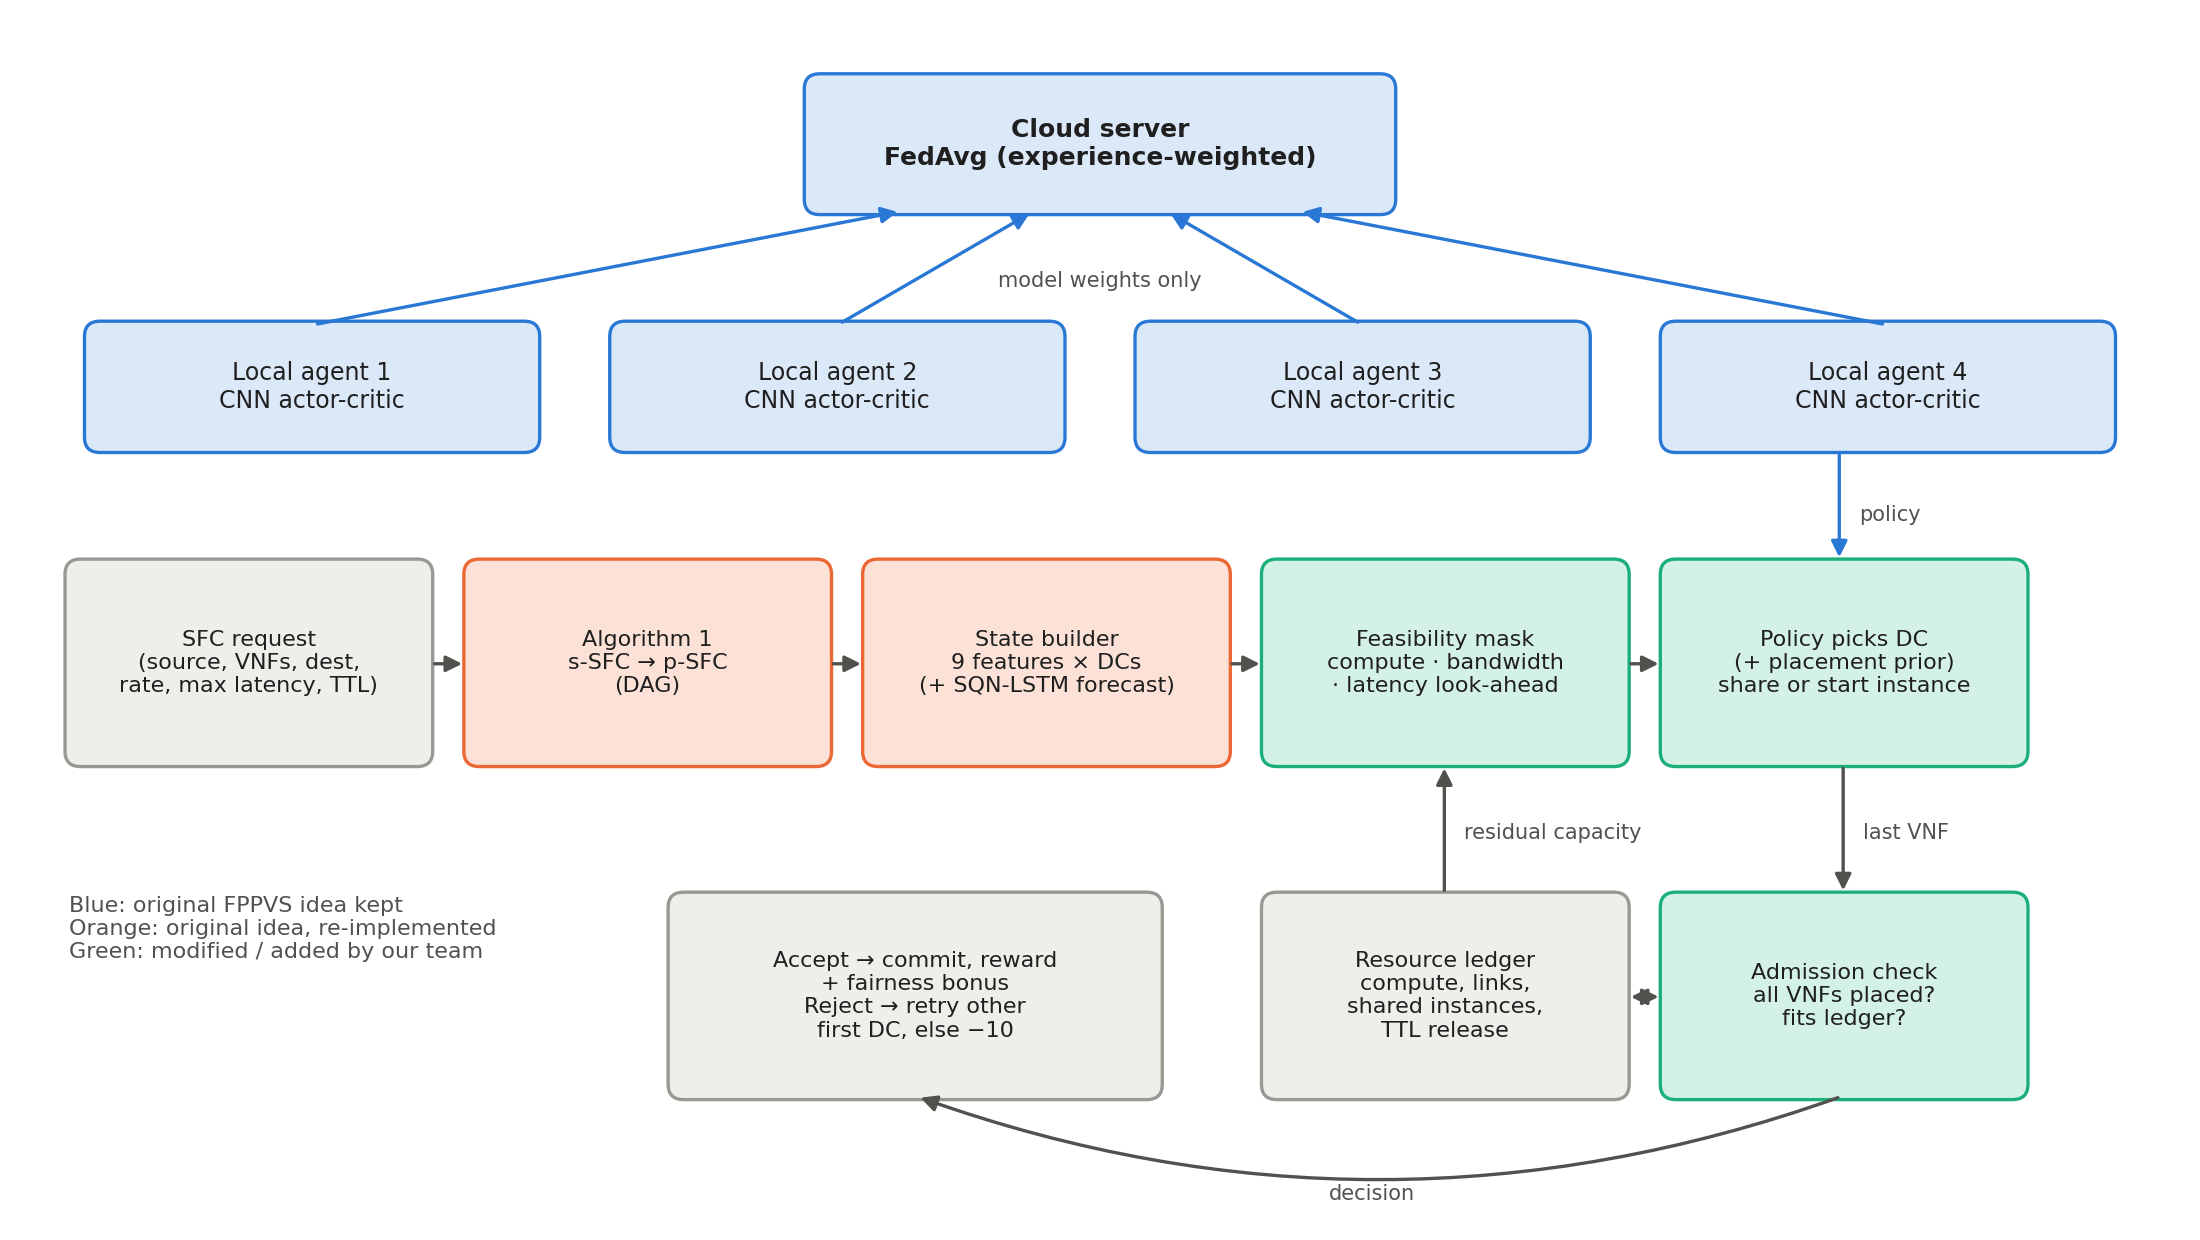
\includegraphics[width=\linewidth]{architecture.png}
\caption{System architecture. A request is turned into a p-SFC, its VNFs are
placed one at a time by a local agent under a feasibility mask, and the
admission check either commits or rejects the whole chain against the resource
ledger. Agents share model weights through FedAvg, never raw request data.}
\label{fig:arch}
\end{figure}

\begin{itemize}
  \item \textbf{Algorithm 1 (s-SFC to p-SFC).} Figure~\ref{fig:psfc} shows what
  our implementation outputs for a five-VNF chain. FW, NAT and LB stay on the
  main chain. IDS branches off after FW and has to join back before NAT, because
  the dependency matrix says so. DPI has no shaper depending on it, so it joins
  back at the destination.
  \item \textbf{State builder and SQN-LSTM.} Builds a grid with one column per DC
  and nine feature rows (Section~\ref{sec:approach}). The SQN keeps the per-type
  demand of the last five requests, and the LSTM predicts the next one.
  \item \textbf{Feasibility mask, policy and admission} are explained in
  Section~\ref{sec:approach}.
  \item \textbf{Resource ledger.} Keeps track of the compute, link bandwidth and
  live shared instances of all active SFCs, frees them when a TTL runs out, and
  adds up resource use over time for the metrics.
  \item \textbf{Federated learning.} Four local agents, each with its own request
  stream and ledger, train locally, and the cloud averages their weights.
\end{itemize}

\begin{figure}[H]
\centering
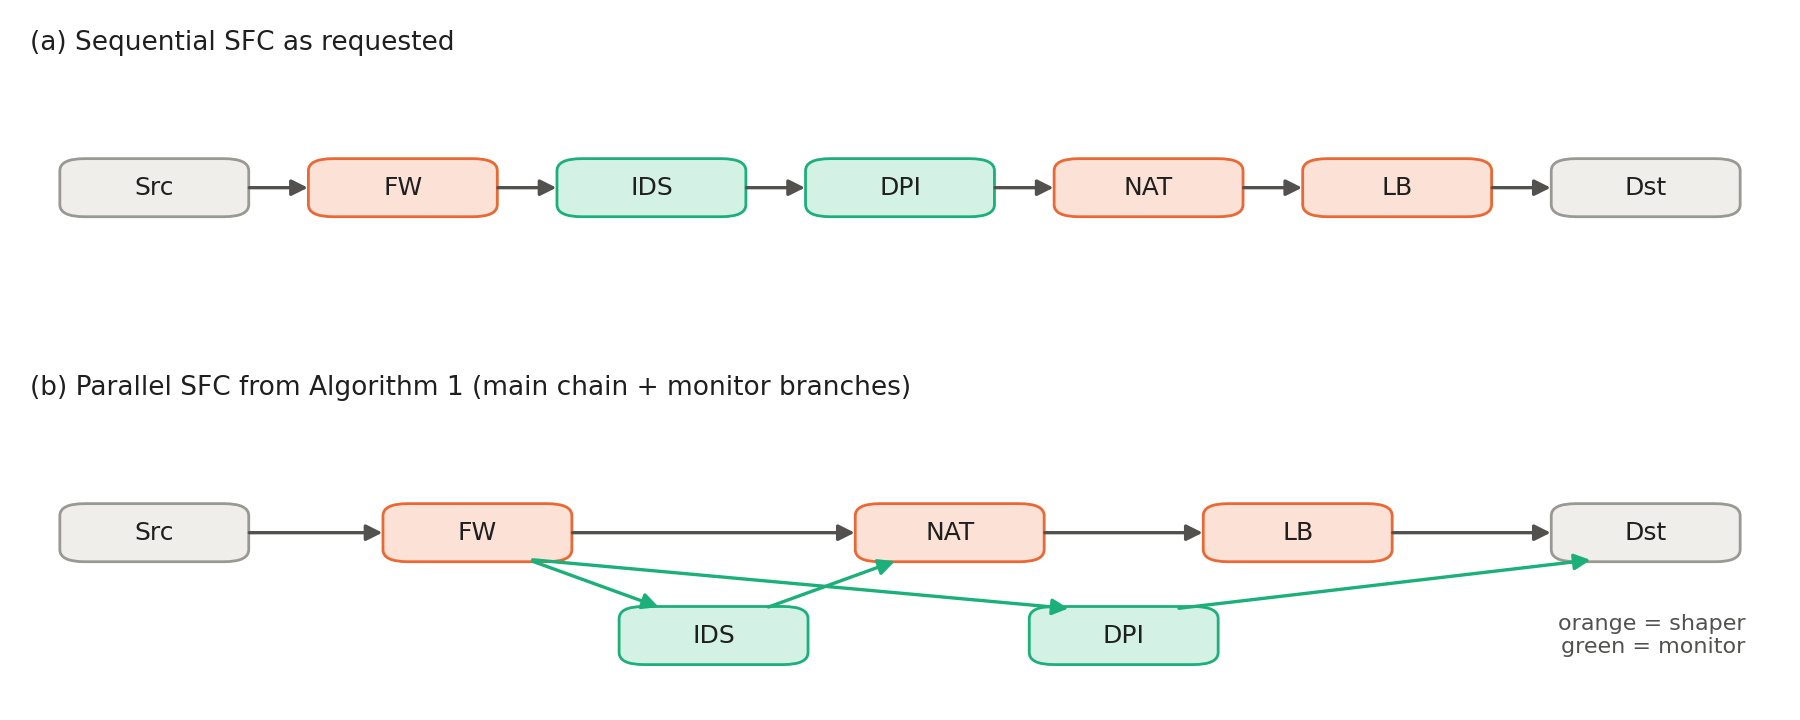
\includegraphics[width=0.9\linewidth]{psfc-example.png}
\caption{Algorithm 1 as we implemented it. Top: the requested sequential chain.
Bottom: the generated p-SFC. IDS has to finish before NAT; DPI has no shaper
depending on it, so it joins back at the destination.}
\label{fig:psfc}
\end{figure}

%=====================================================================
\section{Modified Problem Formulation}
%=====================================================================

\subsection{Original formulation (paper)}
The paper minimizes a weighted sum over time,
\begin{equation}
F_{obj} = \min \sum_{t} \xi_{cost} O_{cost}(t) + \xi_{E2E} O_{E2E}(t)
 - \xi_{acc} O_{acc}(t) - \xi_{utility} O_{utility}(t),
\end{equation}
where $O_{acc}=\frac{1}{|U|}\sum_u y_u$ is the acceptance ratio ($y_u=1$ if
request $u$ is accepted), $O_{cost}$ is the deployment cost, $O_{E2E}$ is the
end-to-end latency and $O_{utility}$ is the $\alpha$-fair throughput utility.
The constraints cover DC capacity, link bandwidth, latency, placement uniqueness
and VNF dependencies.

\subsection{Our modifications}

\paragraph{M1. Explicit offered load (L1).} Requests come in as a Poisson
process with rate $\lambda$, and lifetimes are exponential with mean
$\bar\tau=1000$. We set $\lambda$ from a target offered load
\begin{equation}
\rho = \frac{\lambda\,\bar\tau\,\bar c}{\sum_{i} C_i},
\qquad \bar c = 7\times 0.7 = 4.9,
\end{equation}
where $\bar c$ is the mean compute demand of one SFC (4--10 VNFs of
0.5--0.9 units each). $\rho=1$ means the average offered compute is equal to the
total compute of the network. Our main scenarios use heavy load,
$\rho\in\{0.9, 1.0, 1.1\}$. At light load the problem is kind of easy: at
$\rho=0.5$, almost any placement that keeps chains compact accepts nearly every
request, so light load doesn't really tell us much about the method. We still
report $\rho=0.5$, along with the overload points $\rho\in\{1.25, 1.5\}$, in a
load sweep, so the full range can be seen.

\paragraph{M2. Instance-based compute model (L4).} Each live VNF instance costs a
fixed overhead $o$ (its VM or container footprint, $o=0.25$) plus the demand of
every flow it serves. Let $\mathcal{A}(t)$ be the set of active requests and
$\mathcal{I}_i(t)$ the set of live instances on DC $v_i$. The compute
constraint is
\begin{equation}
\sum_{u\in\mathcal{A}(t)} \sum_{f\in\mathcal{F}_u} c_f\, x^u_{f,i}
\;+\; o\,|\mathcal{I}_i(t)| \;\le\; C_i \qquad \forall v_i, t,
\end{equation}
where $x^u_{f,i}=1$ if VNF $f$ of request $u$ runs on $v_i$. With sharing on, an
instance of type $k$ on $v_i$ gets created by the first VNF of that type and
removed when its last user leaves. Without sharing, every VNF gets its own
instance.

\paragraph{M3. Bandwidth and latency on the p-SFC.} For every virtual edge
$(a,b)$ of the p-SFC, the data rate $r_u$ is reserved on each link of
$P(\pi(a),\pi(b))$, where $\pi$ is the placement:
\begin{equation}
\sum_{u\in\mathcal{A}(t)} \sum_{(a,b)\in E_u} r_u\,
\mathbb{1}\big[(v_i,v_j)\in P(\pi(a),\pi(b))\big] \le B_{ij}.
\end{equation}
The latency of a request is the longest source-to-destination path in the
p-SFC, counting both link latency and VNF processing:
$L_u = \max_{p} \sum_{(a,b)\in p} \big(L_{P(\pi(a),\pi(b))} + \ell_b\big)
\le L^{\max}_u$.

\paragraph{M4. Objective.} The main objective stays the same as in the paper:
maximize $O_{acc}$. As a second objective, we minimize the resources held per
served request over time (L7):
\begin{equation}
R_{comp} = \frac{\int_t \sum_i \mathrm{used}_i(t)\,dt}{\#\text{accepted}},
\qquad
R_{bw} = \frac{\int_t \sum_{(i,j)} \mathrm{used}_{ij}(t)\,dt}{\#\text{accepted}}.
\end{equation}
Latency and fairness come in through the reward (Section~\ref{sec:reward}), just
like in the paper. We don't model monetary cost separately, because with a fixed
price per unit it is proportional to $R_{comp}$ anyway.

%=====================================================================
\section{Proposed Approach}\label{sec:approach}
%=====================================================================

\subsection{Overview}
Each request is one episode. Its VNFs are placed one at a time in their original
order, which is also a topological order of the p-SFC. So when VNF $f$ is put on
a candidate DC, every virtual edge going into $f$ (and its edge to the
destination, if it has one) can already be routed. This is what lets us do an
early feasibility check. Figure~\ref{fig:flow} and Algorithm~\ref{alg:place}
show one decision.

\begin{figure}[H]
\centering
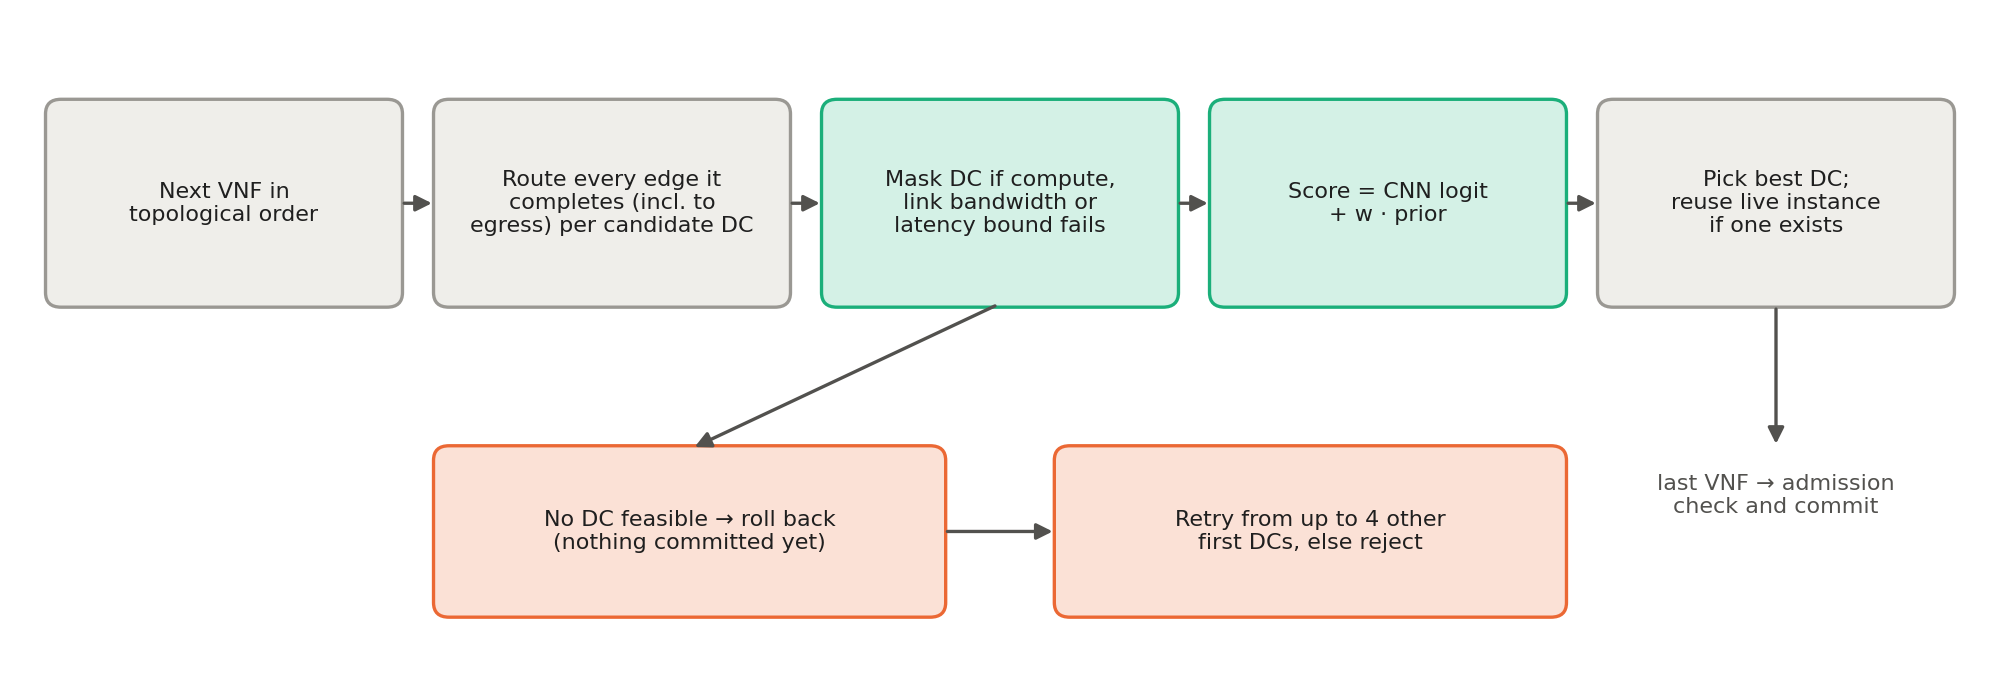
\includegraphics[width=0.95\linewidth]{placement-flow.png}
\caption{One placement decision in the updated FPPVS.}
\label{fig:flow}
\end{figure}

\begin{algorithm}[H]
\caption{Updated FPPVS admission for one request $u$}\label{alg:place}
\begin{algorithmic}[1]
\Require request $u$, ledger $\mathcal{L}$, policy $\pi_\theta$, retries $K$
\State $G_u \gets$ \Call{Parallelize}{$u$} \Comment{Algorithm 1 of the paper}
\For{attempt $= 0,\dots,K$}
  \State reset episode state (nothing is committed yet)
  \For{each VNF $f$ of $u$ in order}
    \For{each DC $v$}
      \State route the edges of $G_u$ completed by putting $f$ on $v$
      \State $m_v \gets$ compute, bandwidth and latency bound all hold
    \EndFor
    \If{no $m_v$ is true} \State \textbf{break} \Comment{dead end, try next attempt} \EndIf
    \If{$f$ is the first VNF and attempt $>0$}
      \State $v^\ast \gets$ the attempt-th best DC by prior score, excluding the policy's choice
    \Else
      \State $v^\ast \gets \arg\max_{v:\,m_v} \big(\text{logit}_\theta(s)_v + w\cdot \text{prior}_v\big)$
    \EndIf
    \State place $f$ on $v^\ast$; reuse a live instance of its type on $v^\ast$ if sharing is on
  \EndFor
  \If{all VNFs placed \textbf{and} \Call{Evaluate}{$G_u$} feasible \textbf{and} fits $\mathcal{L}$}
    \State commit to $\mathcal{L}$ until $t_u+\tau_u$; \Return accept
  \EndIf
\EndFor
\State \Return reject
\end{algorithmic}
\end{algorithm}

\subsection{MDP: state, action and mask}
\textbf{State.} A $9\times|V_s|$ grid, with one column per DC (Table~\ref{tab:state}).

\begin{table}[H]
\centering\small
\caption{State features per DC column. Rows marked ``ours'' were added by us.}
\label{tab:state}
\begin{tabular}{clc}
\toprule
Row & Feature & Origin \\
\midrule
1 & Residual compute fraction (includes all active SFCs) & paper, fixed by us \\
2 & Demand of the current VNF / capacity & paper \\
3 & Latency from the DC of the previous VNF & paper \\
4 & Latency to the destination & \ours{ours} \\
5 & Smallest remaining bandwidth fraction on newly routed links & \ours{ours} \\
6 & A live instance of this VNF type exists (reuse possible) & \ours{ours} \\
7 & SQN-LSTM demand forecast for this VNF type & paper \\
8 & Placement prior score & \ours{ours} \\
9 & Feasibility mask & \ours{ours} \\
\bottomrule
\end{tabular}
\end{table}

\textbf{Action.} Pick one DC for the current VNF. \textbf{Mask.} A DC is
allowed only if (i) its residual compute covers the VNF demand, plus the
instance overhead when a new instance is needed, (ii) every link on the newly
routed paths still has the data rate free, and (iii) the critical-path latency
so far plus the shortest latency from the DC to the destination is within
$L^{\max}_u$. Since shortest-path latency follows the triangle inequality, (iii)
never throws out a DC that could still lead to a valid placement.

\subsection{Placement prior}
The prior score of DC $v$ for VNF $f$ is
\begin{equation}
\begin{split}
\text{prior}_v ={}& -(h^{new}_v + h^{dst}_v) - 2\,\frac{T_v + L(v,d_u)}{L^{\max}_u}
 + 0.5\,\mathbf{1}[\text{reuse}] \\
 & + 0.3\,\mathbf{1}[v = v_{prev}] + 0.5\,\tilde{C}_v - 3\,\frac{\max(0,\,0.25-\beta_v)}{0.25},
\end{split}
\end{equation}
where $h^{new}_v$ is the number of link hops (weighted by data rate) the new
edges use, $h^{dst}_v$ the hops from $v$ to the destination, $T_v$ the
critical-path finish time of $f$ on $v$, $\tilde C_v$ the residual compute
fraction after placement and $\beta_v$ the bandwidth margin. In simple words:
keep the chain short and on a few DCs, reuse live instances, and stay away from
DCs and links that are nearly full.

\subsection{Actor-critic network}
We keep the paper's three convolutional layers with 64 filters, batch
normalization and ReLU, but the kernels are $3\times1$, so they only run along
the feature axis, because columns next to each other are just unrelated DCs. The
\textbf{actor} applies the same two $1\times1$ convolutions to every column,
averages over the feature axis and gives out one logit per DC; on top of that we
add $w\cdot\text{prior}$, where $w$ is a learnable scalar (starting value 2). So
the network learns a correction on top of a sensible rule, and it is
permutation-equivariant: if you reorder the DCs, the outputs get reordered the
same way (a unit test checks this). The \textbf{critic} keeps the paper's
256-unit fully connected layer with dropout 0.3, but we feed it a global average
of the convolution features, so it also works for any number of DCs.

\subsection{Reward}\label{sec:reward}
This follows Eq.~(28) of the paper: $+1$ for each valid placement, $-1$ when a
new instance has to be started, and $-10$ if the request is rejected. We added a
small bandwidth term ($-0.2$ per data-rate-weighted hop) and dropped the paper's
$+5$ reuse bonus, because the prior already rewards reuse. When the request is
accepted, the agent gets $5\,(1 + \max(0,1 - L_u/L^{\max}_u))$, which rewards
latency slack, plus a fairness bonus $5\,\Delta\mathrm{JFI}$ (the change in
Jain's index~\cite{jain} over the throughputs of accepted requests).

\subsection{Training}
Each episode is trained with advantage actor-critic~\cite{a3c}: discounted
returns, advantage = return $-$ critic value, actor loss with an entropy bonus,
critic MSE loss, and gradient clipping. For exploration, we mix the paper's
adaptive $\epsilon$-greedy rule ($\epsilon$ goes down after an accepted request
and goes up after a rejection) with a bit of Gaussian noise on the logits. Four
agents train locally for 50 episodes per round on their own request streams and
ledgers, carrying on through the stream from one round to the next; then the
server averages their weights, weighted by the number of episodes. Evaluation is
deterministic (arg-max over allowed DCs) on a hold-out stream that is never used
for training. Table~\ref{tab:hyper} lists the hyperparameters.

\begin{table}[H]
\centering\small
\caption{Training hyperparameters.}
\label{tab:hyper}
\begin{tabular}{ll@{\qquad}ll}
\toprule
Optimizer & Adam, lr $5\times10^{-4}$ & Discount $\gamma$ & 0.99 \\
Federated agents & 4 & FedAvg rounds & 10 \\
Episodes per agent per round & 50 & Total training episodes & 2000 \\
$\epsilon$ start / min / decay & 0.15 / 0.02 / 0.995 & Logit noise std & 0.10 \\
Entropy coefficient & 0.01 & Gradient clip & 1.0 \\
Critic loss weight & 0.5 & Prior weight $w$ (initial) & 2.0 (learned) \\
SQN depth / LSTM hidden & 5 / 64 & Retries $K$ & 4 \\
Instance overhead $o$ & 0.25 units & Training requests per agent & 600 \\
\bottomrule
\end{tabular}
\end{table}

%=====================================================================
\section{Performance Evaluation}
%=====================================================================

\subsection{Experimental setup}
\textbf{Hardware:} a laptop with a 12th Gen Intel Core i5-12500H CPU and 16 GB of
RAM, running Windows 11. No GPU was used. \textbf{Software:} Python 3.12.1,
PyTorch 2.10 (CPU build), NetworkX 3.6.1 and Matplotlib 3.10.8. Scenarios run in
parallel worker processes, with one PyTorch thread each. Each scenario is
repeated with \numSeeds{} seeds (7--11). For every seed we generate a new
network, four training streams and one hold-out stream. Training one FPPVS model
takes about \trainSeconds\,s.

\begin{table}[H]
\centering\small
\caption{Simulation parameters. Values follow Section 5.1 of the paper unless
marked as ours.}
\label{tab:params}
\begin{tabularx}{\linewidth}{l X}
\toprule
Parameter & Value \\
\midrule
Topologies & Backbone: 24 DCs, 47 links; Metro: 17 DCs, 29 links (random connected graphs) \\
DC compute capacity & $\mathcal{U}(10, 20)$ units \\
Link bandwidth & 100--200 units in steps of 20 \\
Link latency & $\mathcal{U}(5, 20)$ ms \\
SFC length & 4--10 VNFs, types IDS, DPI, LB, FW, NAT \\
Monitor probability (IDS/DPI) & 0.45; a monitor gates a later shaper with prob.\ 0.5 \\
VNF compute demand & $\mathcal{U}(0.5, 0.9)$ units (500--900 Mbps normalized) \\
VNF processing latency & $\mathcal{U}(0.01, 0.2)$ ms \\
Data rate per request & bounded power law on $[5, 30]$, exponent 1.5 \\
Maximum latency & $\mathcal{U}(100, 150)$ ms \\
Lifetime (TTL) & exponential, mean 1000 time units \\
Arrivals & \ours{Poisson, rate set by offered load $\rho$} \\
Offered load $\rho$ & \ours{0.9, 1.0, 1.1 (main); 0.5, 1.25, 1.5 (load sweep)} \\
Instance overhead & \ours{0.25 units per live instance} \\
Requests per stream & \ours{600 hold-out; 600 per training agent} \\
\bottomrule
\end{tabularx}
\end{table}

\subsection{Performance metrics}
\begin{itemize}
  \item \textbf{Service acceptance}: accepted hold-out requests divided by all
  hold-out requests (higher is better).
  \item \textbf{Compute / bandwidth per running SFC}: time-averaged compute (or
  bandwidth) in use divided by the time-averaged number of running SFCs. This is
  basically how much resource one service is holding at any moment (lower is
  better).
  \item \textbf{Compute$\cdot$time and bandwidth$\cdot$time per accepted SFC}:
  $R_{comp}$ and $R_{bw}$ from Section 4 (lower is better).
  \item \textbf{Instances per accepted SFC}: VNF instances started divided by
  accepted requests; this shows how much sharing is going on (lower is better).
  \item \textbf{Latency}: mean critical-path end-to-end latency of accepted
  requests.
  \item \textbf{Decision time}: wall-clock time per request, retries included.
\end{itemize}

\subsection{Compared methods}
We compare five methods. All of them run in the same simulator, on the same
networks, training streams and hold-out requests, with the same instance model
(M2), so none of them can overbook capacity. The three learning methods get the
same training budget of 2000 episodes.
\begin{itemize}
  \item \textbf{Updated FPPVS (ours):} the method from Section~\ref{sec:approach}.
  \item \textbf{Original FPPVS} (Zhu et al.~\cite{fppvs}), implemented as
  close as we could get to Section 4.3 of the paper. Resource-aware pruning
  throws out DCs that don't have enough compute or free bandwidth on the links
  the next hop would use; the next VNF goes on the current node or a
  neighbouring node; the state holds residual capacity, VNF demand, distance
  from the previous VNF, the SQN-LSTM forecast, whether a DC already hosts this
  VNF type (the paper's history-based prioritisation) and the pruned candidate
  set. The network is the paper's CNN (three $3\times3$ convolution layers with
  64 filters and batch normalization, the feature map as a fixed-length vector
  into a 256-unit layer with dropout 0.3, one output per DC). It uses the paper's
  step reward (Eq.~28: $+1$ valid, $+5$ reuse, $-1$ new instance, $-10$
  rejection), adaptive $\epsilon$-greedy exploration and federated training (4
  agents, 10 rounds, 50 episodes). It has no latency look-ahead, no placement
  prior and no retries, because those are things we added.
  \item \textbf{2022 adaptation} of Zhang et al.~\cite{zhang2022}: online SFC
  placement with sequential VNF placement (no parallelization), reuse of an
  existing VNF of the same type, an SQN-LSTM queue of depth $T_D=20$ for demand
  forecasting, an actor-critic placement policy (a fully connected network over
  the same four-row state), and rollback when a request can't be completed.
  Its reward follows the long-term revenue-to-cost ratio (LTCR): on success the
  agent gets $10\cdot\min(2,\ \text{revenue}/\text{cost})$, where revenue is
  the requested compute plus bandwidth and cost is the compute and link
  bandwidth actually used; a failure gets a fixed penalty of $-10$. It is
  trained by a single synchronous agent. This is our own adaptation from the
  method description, since the authors' code was not available.
  \item \textbf{Greedy:} the feasible DC with the most residual compute (load
  balancing), without sharing.
  \item \textbf{Random:} a random feasible DC, without sharing.
\end{itemize}
Greedy and random use our feasibility mask, so they never pick a DC that is
already known to be infeasible. We also compare against the numbers published in
the FPPVS paper (Section~\ref{sec:paper}). On top of that, an ablation study
turns off one part of updated FPPVS at a time (no sharing, no fairness bonus, a
single agent, no retries, and the placement prior alone with no learning).

\subsection{Results}

% Results section, included from report.tex. All tables are generated by
% scripts/make_report_tables.py from output/scenarios/scenario-results.json.

\subsubsection*{A. Service acceptance}

Table~\ref{tab:acc} and Figure~\ref{fig:acc} give the hold-out acceptance for
every scenario. The main scenarios are all heavy load: offered demand at 90\%,
100\% and 110\% of the network's compute capacity. Updated FPPVS hits the 70\%
target in all six main scenarios. Its mean acceptance goes from \fppvsMinAcc\%
(\fppvsWorstScenario) to \fppvsMaxAcc\%, with an average of \fppvsMeanAcc\%. The
lowest value in any single seed was \fppvsLowestRun\%, so the target holds run
by run too, not just on average.

\begin{table}[H]
\centering\footnotesize
\setlength{\tabcolsep}{4pt}
\caption{Hold-out service acceptance (\%), mean $\pm$ standard deviation over
\numSeeds{} seeds. Best value per row in bold.}
\label{tab:acc}
\begin{tabular}{lccccc}
\toprule
Scenario (topology, load) & Updated (ours) & Original FPPVS & 2022 adaptation & Greedy & Random \\
\midrule
Backbone 0.9 & \textbf{91.0 $\pm$ 3.6} & 77.0 $\pm$ 2.1 & 47.8 $\pm$ 7.6 & 58.7 $\pm$ 4.4 & 57.4 $\pm$ 4.0 \\
Backbone 1 & \textbf{86.4 $\pm$ 3.7} & 72.9 $\pm$ 2.4 & 44.5 $\pm$ 6.5 & 53.4 $\pm$ 5.1 & 55.3 $\pm$ 3.4 \\
Backbone 1.1 & \textbf{80.8 $\pm$ 3.8} & 67.7 $\pm$ 3.1 & 43.0 $\pm$ 10.4 & 51.9 $\pm$ 4.9 & 52.9 $\pm$ 3.3 \\
Metro 0.9 & \textbf{86.1 $\pm$ 2.9} & 73.6 $\pm$ 3.6 & 53.1 $\pm$ 9.3 & 56.3 $\pm$ 3.1 & 56.6 $\pm$ 3.0 \\
Metro 1 & \textbf{81.3 $\pm$ 3.5} & 69.6 $\pm$ 3.6 & 49.4 $\pm$ 9.7 & 51.8 $\pm$ 3.6 & 52.6 $\pm$ 3.0 \\
Metro 1.1 & \textbf{76.6 $\pm$ 2.5} & 65.6 $\pm$ 3.2 & 50.1 $\pm$ 5.2 & 48.8 $\pm$ 1.9 & 50.9 $\pm$ 3.1 \\
\midrule \multicolumn{6}{l}{\emph{Other load levels (light load and overload)}} \\
Backbone 0.5 & \textbf{99.6 $\pm$ 0.4} & 91.2 $\pm$ 2.3 & 68.1 $\pm$ 5.4 & 72.1 $\pm$ 5.8 & 73.2 $\pm$ 4.5 \\
Backbone 1.25 & \textbf{75.2 $\pm$ 2.9} & 65.5 $\pm$ 2.7 & 41.1 $\pm$ 3.0 & 49.3 $\pm$ 3.8 & 50.9 $\pm$ 2.7 \\
Backbone 1.5 & \textbf{65.2 $\pm$ 3.3} & 58.2 $\pm$ 3.2 & 38.4 $\pm$ 4.3 & 43.4 $\pm$ 4.1 & 44.2 $\pm$ 2.1 \\
Metro 0.5 & \textbf{99.0 $\pm$ 0.8} & 89.2 $\pm$ 3.7 & 74.0 $\pm$ 9.7 & 71.4 $\pm$ 3.0 & 72.1 $\pm$ 2.9 \\
Metro 1.25 & \textbf{69.2 $\pm$ 4.2} & 61.1 $\pm$ 3.7 & 40.5 $\pm$ 7.8 & 47.2 $\pm$ 2.1 & 46.9 $\pm$ 2.3 \\
Metro 1.5 & \textbf{60.6 $\pm$ 1.9} & 53.3 $\pm$ 5.2 & 42.2 $\pm$ 3.9 & 42.2 $\pm$ 2.7 & 43.1 $\pm$ 1.3 \\
\bottomrule
\end{tabular}
\end{table}

\begin{figure}[H]
\centering
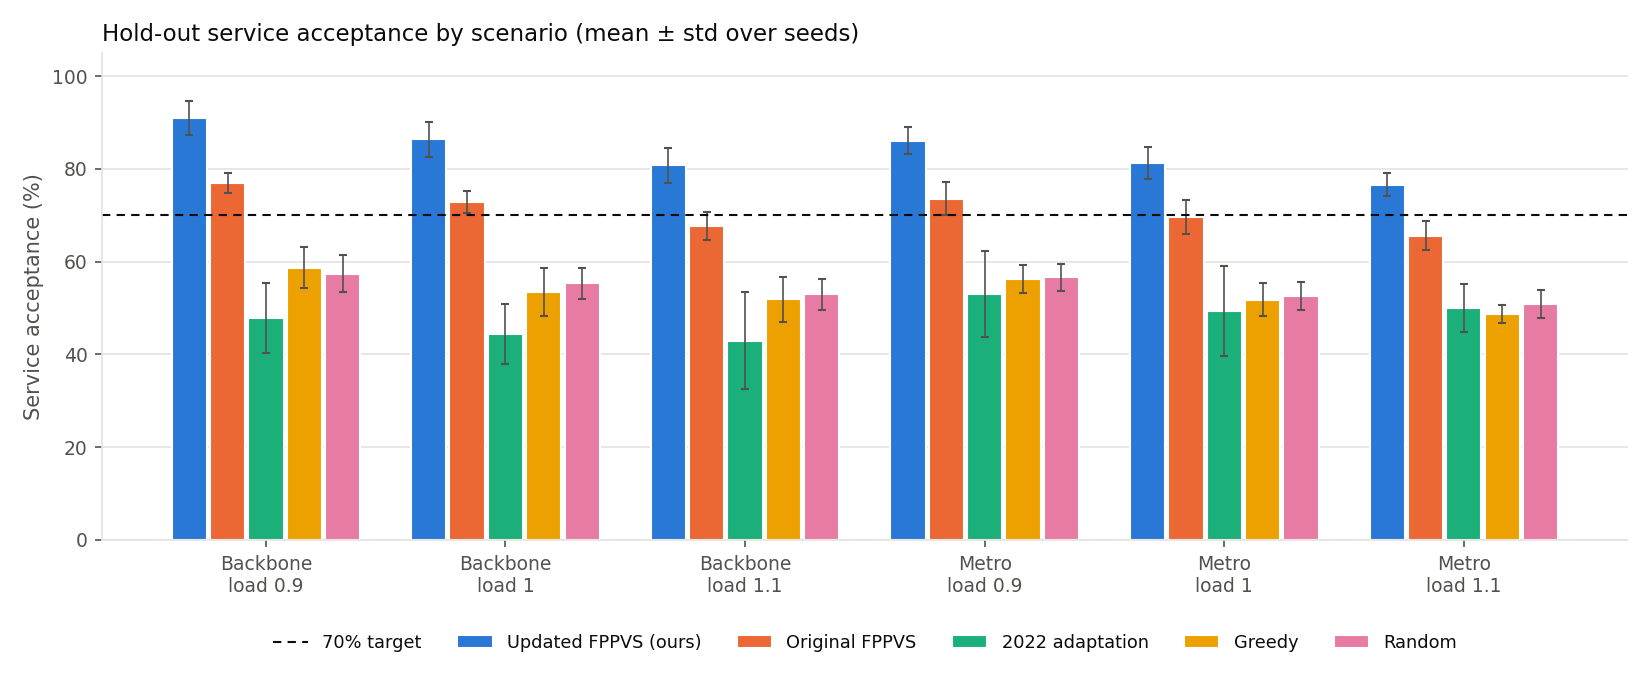
\includegraphics[width=\linewidth]{scenario-acceptance.png}
\caption{Hold-out acceptance in the six main scenarios. Error bars show one
standard deviation over seeds; the dashed line is the 70\% target.}
\label{fig:acc}
\end{figure}

\needspace{5\baselineskip}
\paragraph{Observations.}
\begin{itemize}
  \item Updated FPPVS is the best method in every scenario. At full load
  ($\rho=1$) it accepts 86.4\% on Backbone and 81.3\% on Metro, and even at 10\%
  overload ($\rho=1.1$) it still gets 80.8\% and 76.6\%.
  \item The original FPPVS is clearly second. It reaches
  \origMinAcc--\origMaxAcc\% in the main scenarios (mean \origMeanAcc\%) and
  beats the 2022 adaptation, greedy and random in every scenario, and in every
  one of the 30 main-scenario runs too; per scenario, its lead over the best of
  those three is 15--18 points. Its bandwidth pruning and neighbour rule keep
  chains compact, and its history signal pushes VNFs towards DCs that already
  run the same type. Updated FPPVS is \origGainMin--\origGainMax{} points above
  it (\origGainMean{} on average).
  \item The 2022 adaptation gets only \zhangMinAcc--\zhangMaxAcc\% (mean
  \zhangMeanAcc\%), which is below greedy and random in most scenarios. Greedy
  and random run with our feasibility mask, so they never pick a DC that is
  already known to break bandwidth or latency. The 2022 adaptation only checks
  compute while placing, as its method describes, and finds out about bandwidth
  and latency violations only when the whole chain is done (see Part E).
  \item The 2022 adaptation is also the least stable method: its standard
  deviation across seeds goes up to 10 points (Backbone, $\rho=1.1$). Getting
  just one reward value per episode (LTCR) gives the agent a weak learning
  signal.
  \item Greedy and random accept 49--59\%. They spread VNFs over a lot of DCs, so
  each request uses about twice as much link bandwidth as updated FPPVS
  (Section~C), and the links run out first.
  \item Metro is harder than Backbone at the same load. It has fewer DCs and
  fewer links, so when a link fills up there just aren't many other paths to
  use.
\end{itemize}

\begin{figure}[H]
\centering
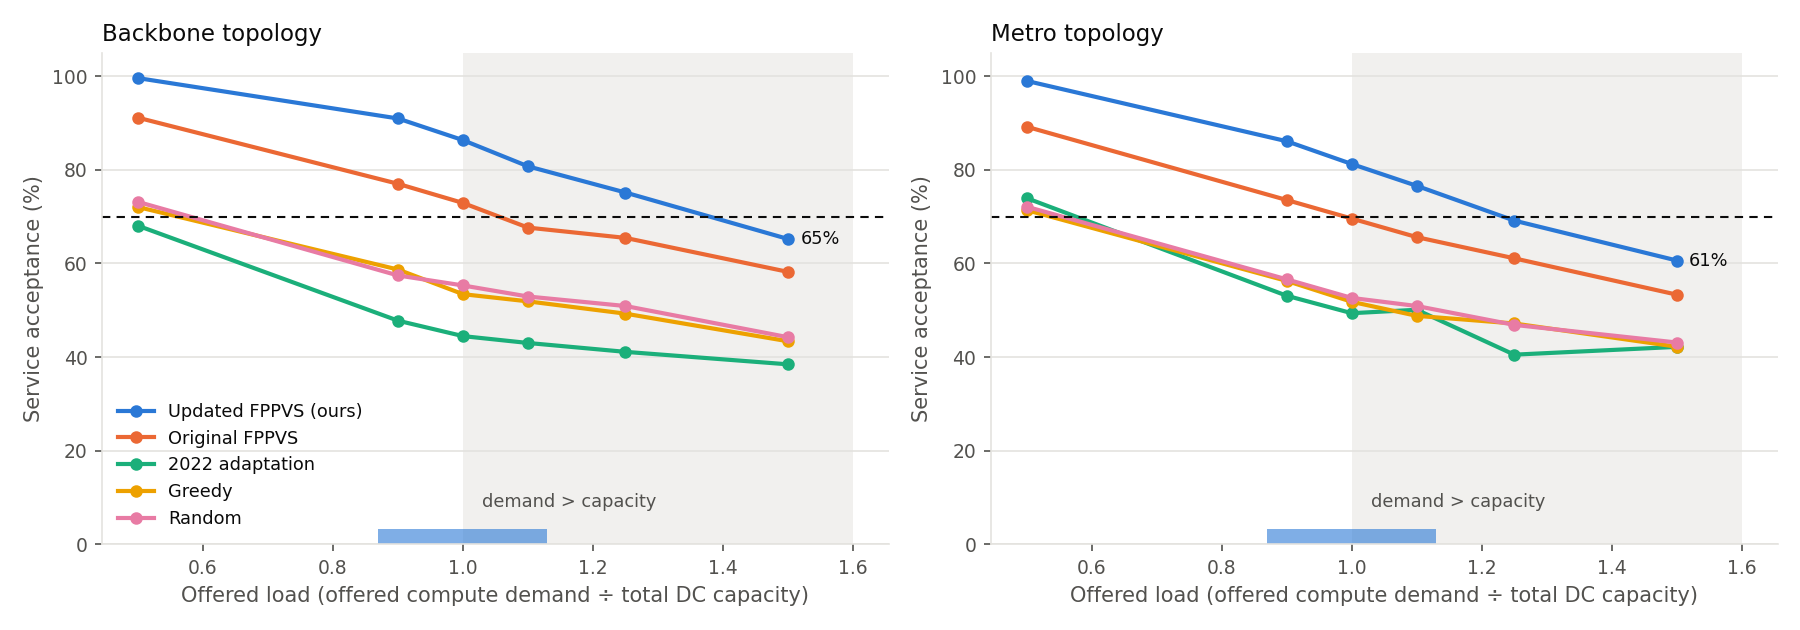
\includegraphics[width=\linewidth]{load-sweep.png}
\caption{Acceptance against offered load, from light load (0.5) to 50\%
overload (1.5). The shaded area is where the average offered compute is more
than the total compute of the network; the blue mark on the x-axis shows the
main scenarios.}
\label{fig:sweep}
\end{figure}

\paragraph{Load sweep.} Figure~\ref{fig:sweep} shows the full range of loads. At
light load ($\rho=0.5$), updated FPPVS accepts 99.6\% (Backbone) and 99.0\%
(Metro). This is kind of expected: with the network only half full, almost
every request fits as long as chains are kept compact, and the original FPPVS
also gets 91.2\% and 89.2\% there. That's why we use heavier loads as the main
scenarios. As the load goes up, acceptance drops smoothly: updated FPPVS gets
75.2\% and 69.2\% at $\rho=1.25$, and 65.2\% and 60.6\% at $\rho=1.5$. The
original FPPVS follows 7--10 points lower (53--66\%), and the 2022 adaptation,
greedy and random stay at or below 51\%. Going below 70\% can't be avoided in
this region: at $\rho=1.5$, only about two thirds of the offered compute can fit
in the network at any time, no matter what the placement policy is.

\subsubsection*{B. Ablation study}

\begin{table}[H]
\centering\small
\caption{Ablation: hold-out acceptance (\%) of updated FPPVS with one part
switched off at a time.}
\label{tab:ablation}
\begin{tabular}{lcccccc}
\toprule
Scenario & Full & w/o sharing & w/o fairness & 1 agent & w/o retry & Prior only \\
\midrule
Backbone 0.9 & 91.0 $\pm$ 3.6 & 78.7 $\pm$ 3.7 & 91.4 $\pm$ 3.2 & 90.9 $\pm$ 2.0 & 90.9 $\pm$ 2.8 & 91.9 $\pm$ 3.1 \\
Backbone 1 & 86.4 $\pm$ 3.7 & 73.8 $\pm$ 3.1 & 85.6 $\pm$ 3.9 & 86.0 $\pm$ 3.4 & 85.4 $\pm$ 3.1 & 86.3 $\pm$ 2.8 \\
Backbone 1.1 & 80.8 $\pm$ 3.8 & 68.2 $\pm$ 2.7 & 80.4 $\pm$ 4.1 & 81.2 $\pm$ 3.2 & 80.2 $\pm$ 3.5 & 80.9 $\pm$ 3.0 \\
Metro 0.9 & 86.1 $\pm$ 2.9 & 76.1 $\pm$ 2.1 & 86.8 $\pm$ 3.1 & 86.2 $\pm$ 3.0 & 86.0 $\pm$ 2.9 & 86.1 $\pm$ 3.1 \\
Metro 1 & 81.3 $\pm$ 3.5 & 70.6 $\pm$ 3.2 & 81.1 $\pm$ 2.9 & 81.0 $\pm$ 3.2 & 81.9 $\pm$ 4.0 & 81.7 $\pm$ 3.2 \\
Metro 1.1 & 76.6 $\pm$ 2.5 & 64.5 $\pm$ 2.8 & 75.7 $\pm$ 3.8 & 75.9 $\pm$ 3.8 & 76.4 $\pm$ 3.7 & 76.4 $\pm$ 2.9 \\
\bottomrule
\end{tabular}
\end{table}

Table~\ref{tab:ablation} turns off one part of updated FPPVS at a time.
\begin{itemize}
  \item \textbf{VNF sharing matters the most.} Without it, acceptance drops by
  10--13 points in every main scenario (for example 86.4\% to 73.8\% on Backbone
  at $\rho=1$). Every VNF then pays its own instance overhead, so the DCs fill up
  sooner.
  \item \textbf{Fairness bonus, single vs.\ federated training and retries}
  change acceptance by about one point or less, which is within the
  seed-to-seed spread. Fairness is meant to balance throughput between flows,
  not to push acceptance up, so this is expected. Retries only help in the rare
  case where the first placement runs into a dead end.
  \item \textbf{The learned network adds little over its prior.} ``Prior only''
  uses the same mask, prior and retries with no neural network at all, and it is
  within about one point of the full method everywhere. We're reporting this
  openly: in our experiments, the gains mostly come from the problem
  modifications (mask, sharing model, prior), not from the reinforcement
  learning itself. One reason is limitation L6: each episode covers only one
  request, so the agent doesn't see much of the long-term effect of its choices.
\end{itemize}

\subsubsection*{C. Resource usage}

Figure~\ref{fig:res} and Table~\ref{tab:res} show the resources each method holds
for the services it runs. Table~\ref{tab:savings} sums up the difference
between updated FPPVS and each of the other methods, averaged over the six main
scenarios.

\begin{figure}[H]
\centering
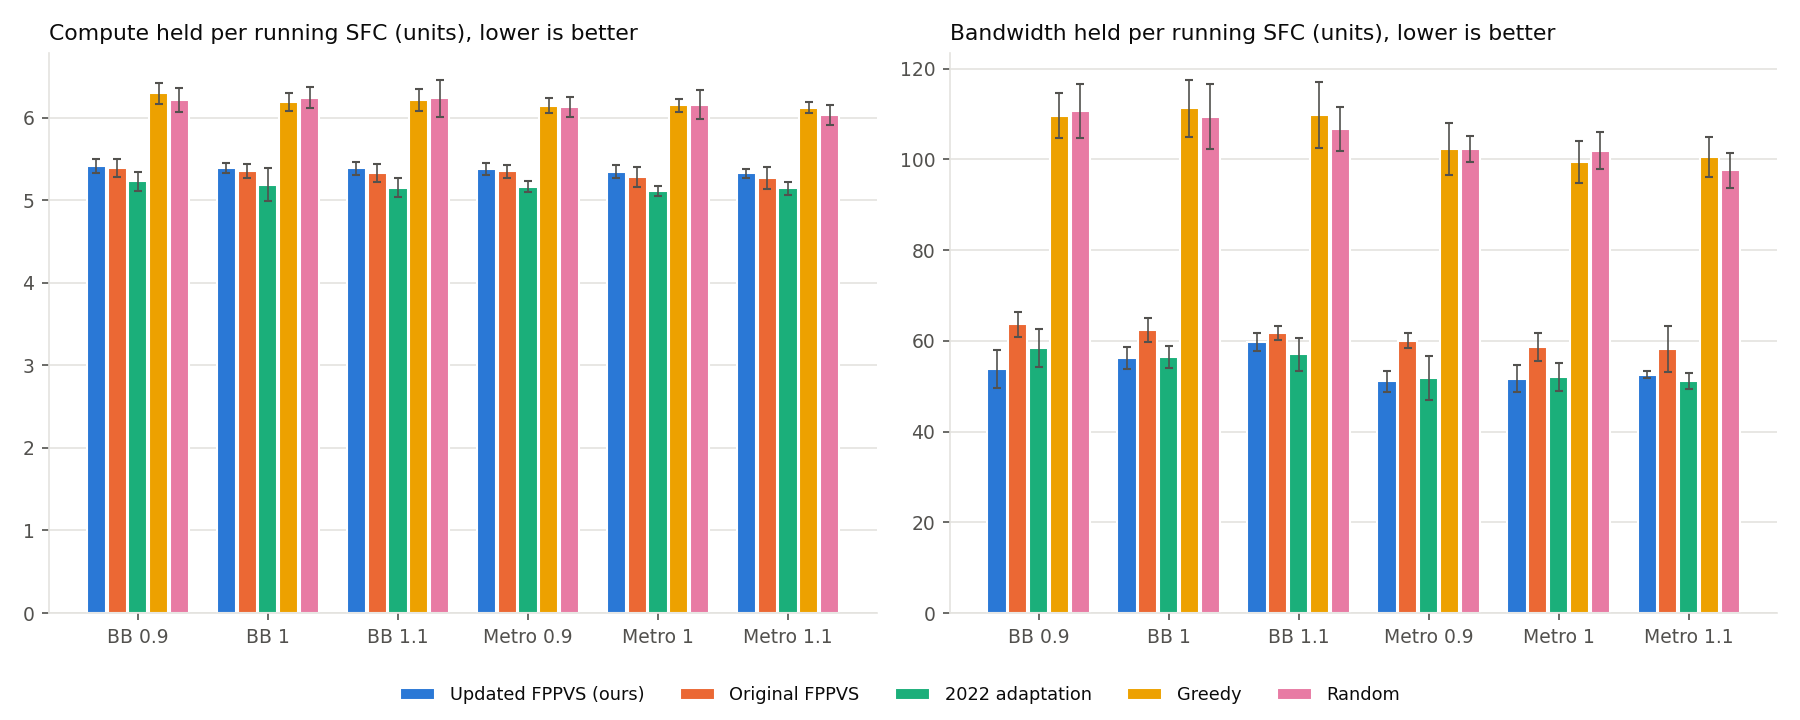
\includegraphics[width=\linewidth]{scenario-resources.png}
\caption{Compute (left) and bandwidth (right) held per running SFC, averaged over
time. Lower means each service costs less to keep running.}
\label{fig:res}
\end{figure}

\begin{table}[H]
\centering\small
\caption{Average reduction in resource use by updated FPPVS over each
method (main scenarios; positive means updated FPPVS uses less, negative means
it uses more).}
\label{tab:savings}
\begin{tabular}{lcccc}
\toprule
Reduction vs. & Compute & Bandwidth & BW$\cdot$time & Instances \\
 & per SFC & per SFC & per accepted & per accepted \\
\midrule
Original FPPVS & -0.8\% & +10.9\% & +11.0\% & +27.0\% \\
2022 adaptation & -4.0\% & +0.5\% & +2.1\% & +13.7\% \\
Greedy & +13.1\% & +48.7\% & +49.4\% & +91.8\% \\
Random & +12.9\% & +48.3\% & +48.6\% & +91.8\% \\
\bottomrule
\end{tabular}
\end{table}

\begin{table}[H]
\centering\scriptsize
\setlength{\tabcolsep}{4pt}
\caption{Resource use and latency per scenario (mean over seeds; best per
column within a scenario in bold). ``Per acc.'' means per accepted SFC.}
\label{tab:res}
\begin{tabular}{llcccccc}
\toprule
Scenario & Method & Compute & Bandwidth & Compute$\cdot$time & BW$\cdot$time & Instances & Latency \\
 & & per SFC & per SFC & per acc. ($10^3$) & per acc. ($10^3$) & per acc. & (ms) \\
\midrule
Backbone 0.9 & Updated (ours) & 5.42 & \textbf{53.8} & 5.43 & \textbf{54.0} & \textbf{0.57} & \textbf{46.5} \\
 & Original FPPVS & 5.39 & 63.7 & \textbf{5.32} & 62.9 & 0.78 & 56.0 \\
 & 2022 adaptation & \textbf{5.23} & 58.4 & 5.37 & 60.0 & 0.59 & 66.2 \\
 & Greedy & 6.29 & 109.6 & 6.31 & 109.8 & 6.66 & 107.8 \\
 & Random & 6.22 & 110.7 & 6.40 & 114.0 & 6.57 & 108.8 \\
\midrule
Backbone 1 & Updated (ours) & 5.39 & \textbf{56.2} & 5.42 & \textbf{56.5} & \textbf{0.53} & \textbf{50.0} \\
 & Original FPPVS & 5.35 & 62.3 & 5.40 & 62.9 & 0.73 & 56.2 \\
 & 2022 adaptation & \textbf{5.19} & 56.5 & \textbf{5.28} & 57.4 & 0.61 & 67.2 \\
 & Greedy & 6.19 & 111.2 & 6.40 & 115.1 & 6.58 & 107.7 \\
 & Random & 6.24 & 109.4 & 6.27 & 110.1 & 6.58 & 108.1 \\
\midrule
Backbone 1.1 & Updated (ours) & 5.39 & 59.6 & 5.40 & 59.9 & \textbf{0.52} & \textbf{53.2} \\
 & Original FPPVS & 5.33 & 61.7 & 5.37 & 62.2 & 0.74 & 54.7 \\
 & 2022 adaptation & \textbf{5.15} & \textbf{57.0} & \textbf{5.26} & \textbf{58.2} & 0.63 & 70.2 \\
 & Greedy & 6.21 & 109.9 & 6.30 & 111.5 & 6.59 & 107.4 \\
 & Random & 6.23 & 106.7 & 6.24 & 107.0 & 6.56 & 108.8 \\
\midrule
Metro 0.9 & Updated (ours) & 5.38 & \textbf{51.1} & 5.50 & \textbf{52.3} & \textbf{0.55} & \textbf{45.8} \\
 & Original FPPVS & 5.35 & 60.0 & 5.44 & 61.1 & 0.74 & 54.5 \\
 & 2022 adaptation & \textbf{5.17} & 51.8 & \textbf{5.28} & 53.1 & 0.67 & 65.5 \\
 & Greedy & 6.15 & 102.2 & 6.27 & 104.6 & 6.56 & 105.2 \\
 & Random & 6.13 & 102.2 & 6.22 & 103.9 & 6.47 & 105.9 \\
\midrule
Metro 1 & Updated (ours) & 5.35 & \textbf{51.6} & 5.44 & \textbf{52.5} & \textbf{0.55} & \textbf{48.6} \\
 & Original FPPVS & 5.28 & 58.7 & 5.46 & 60.7 & 0.71 & 54.1 \\
 & 2022 adaptation & \textbf{5.11} & 52.0 & \textbf{5.35} & 54.4 & 0.62 & 67.2 \\
 & Greedy & 6.15 & 99.4 & 6.46 & 104.4 & 6.53 & 104.1 \\
 & Random & 6.16 & 101.9 & 6.38 & 105.6 & 6.51 & 105.2 \\
\midrule
Metro 1.1 & Updated (ours) & 5.33 & 52.6 & 5.43 & 53.6 & \textbf{0.51} & \textbf{50.2} \\
 & Original FPPVS & 5.28 & 58.3 & 5.37 & 59.3 & 0.71 & 54.2 \\
 & 2022 adaptation & \textbf{5.14} & \textbf{51.2} & \textbf{5.32} & \textbf{53.0} & 0.63 & 65.2 \\
 & Greedy & 6.12 & 100.5 & 6.34 & 104.1 & 6.52 & 105.0 \\
 & Random & 6.03 & 97.6 & 6.14 & 99.4 & 6.41 & 104.0 \\
\bottomrule
\end{tabular}
\end{table}

\needspace{5\baselineskip}
\paragraph{Observations.}
\begin{itemize}
  \item \textbf{Coming to bandwidth:} updated FPPVS holds about half the link
  bandwidth per running SFC compared to greedy and random (48--49\% less), and
  11\% less than the original FPPVS. Against the 2022 adaptation it's about
  even: 0.5\% less on average, lower at $\rho=0.9$ and $\rho=1.0$, and a bit
  higher at $\rho=1.1$. But keep in mind that updated FPPVS carries 1.5--1.9
  times as many requests as the 2022 adaptation at the same time, including
  harder ones that the other method rejects.
  \item \textbf{Coming to instances:} updated FPPVS starts 0.51--0.57 new VNF
  instances per accepted request. That is 27\% fewer than the original FPPVS
  (0.71--0.78), 14\% fewer than the 2022 adaptation, and about 92\% fewer than
  greedy and random (about 6.6, one per VNF, since they don't share). The
  placement prior's reuse term is the main reason for this.
  \item \textbf{Coming to compute:} against greedy and random, it needs about
  13\% less compute per service, because it shares instances. Against the
  original FPPVS it's about the same (within 1\%). Against the 2022 adaptation
  it uses about 4\% more. But that method accepts far fewer requests, most
  likely the easier ones, so its per-request average comes from an easier set.
  \item \textbf{Coming to latency:} mean latency of accepted requests is
  46--53\,ms for updated FPPVS, 54--56\,ms for the original FPPVS, 65--70\,ms for
  the 2022 adaptation, and 104--108\,ms for greedy and random. All of them are
  under the 100--150\,ms limits. The 2022 adaptation places the chain strictly in
  sequence (no parallel branches), so every monitor adds to the critical path.
  \item \textbf{Decision time and training.} Updated FPPVS needs 9--13\,ms per
  request, including the CNN forward pass and the occasional retry; the original
  FPPVS needs 17--28\,ms, because its fully connected layer takes in the whole
  feature map; the 2022 adaptation needs 4--5\,ms; and greedy and random need
  2--3\,ms. Training one updated FPPVS model with 2000 episodes takes about
  \trainSeconds\,s on the CPU, and one original FPPVS model takes about
  200--400\,s.
\end{itemize}

\subsubsection*{D. Effect of the algorithm alone}

Our main experiments use a different arrival process from our first version
(modification M1). So to separate the effect of the algorithm from the effect of
the workload, we also ran the updated placement logic on the original workload:
one arrival per time unit, 100 requests, with almost nothing released during the
run (Table~\ref{tab:old}). The updated placement gets 70.4\%, up from 10.4\% for
the original implementation. Acceptance is lower than in the Poisson runs mainly
because the original stream throws far more traffic at the network than it can
hold.

\begin{table}[H]
\centering\small
\caption{Original workload (one arrival per time unit), 5 seeds. The upper
rows are from our first implementation; the lower rows use the updated
environment and placement logic.}
\label{tab:old}
\begin{tabular}{lc}
\toprule
Method (original workload, 100 requests) & Acceptance (\%) \\
\midrule
Original implementation, trained FDRL (5 seeds) & 10.4 $\pm$ 5.1 \\
Original implementation, greedy & 15.8 $\pm$ 3.1 \\
Original implementation, random & 11.6 $\pm$ 3.0 \\
\midrule
Updated FPPVS placement & 70.4 $\pm$ 2.9 \\
Greedy & 45.4 $\pm$ 2.1 \\
Random & 46.2 $\pm$ 2.2 \\
\bottomrule
\end{tabular}
\end{table}

\subsubsection*{E. Comparison with the original FPPVS and the 2022 adaptation}\label{sec:paper}

\paragraph{Same scenarios, same requests.} Table~\ref{tab:orig} puts the three
learning-based methods side by side. All three get 2000 training episodes and
are tested on the same hold-out requests.

\begin{table}[H]
\centering\small
\caption{Original FPPVS, the 2022 adaptation and updated FPPVS on identical
scenarios, mean over \numSeeds{} seeds. $^\ast$Gain = updated FPPVS minus the
better of the other two, in percentage points.}
\label{tab:orig}
\begin{tabular}{lccccccc}
\toprule
 & \multicolumn{4}{c}{Acceptance (\%)} & \multicolumn{3}{c}{Bandwidth per running SFC} \\
\cmidrule(lr){2-5}\cmidrule(lr){6-8}
Scenario & Original & 2022 & Updated & Gain$^\ast$ & Original & 2022 & Updated \\
\midrule
Backbone 0.9 & 77.0 & 47.8 & \textbf{91.0} & +14.0 & 63.7 & 58.4 & \textbf{53.8} \\
Backbone 1 & 72.9 & 44.5 & \textbf{86.4} & +13.4 & 62.3 & 56.5 & \textbf{56.2} \\
Backbone 1.1 & 67.7 & 43.0 & \textbf{80.8} & +13.1 & 61.7 & 57.0 & \textbf{59.6} \\
Metro 0.9 & 73.6 & 53.1 & \textbf{86.1} & +12.6 & 60.0 & 51.8 & \textbf{51.1} \\
Metro 1 & 69.6 & 49.4 & \textbf{81.3} & +11.7 & 58.7 & 52.0 & \textbf{51.6} \\
Metro 1.1 & 65.6 & 50.1 & \textbf{76.6} & +11.0 & 58.3 & 51.2 & \textbf{52.6} \\
\midrule \multicolumn{8}{l}{\emph{Other load levels}} \\
Backbone 0.5 & 91.2 & 68.1 & \textbf{99.6} & +8.5 & 65.5 & 57.6 & \textbf{40.5} \\
Backbone 1.25 & 65.5 & 41.1 & \textbf{75.2} & +9.7 & 61.1 & 57.1 & \textbf{59.9} \\
Backbone 1.5 & 58.2 & 38.4 & \textbf{65.2} & +7.0 & 60.1 & 57.8 & \textbf{59.5} \\
Metro 0.5 & 89.2 & 74.0 & \textbf{99.0} & +9.8 & 60.5 & 52.9 & \textbf{41.0} \\
Metro 1.25 & 61.1 & 40.5 & \textbf{69.2} & +8.1 & 58.8 & 52.2 & \textbf{55.4} \\
Metro 1.5 & 53.3 & 42.2 & \textbf{60.6} & +7.3 & 58.6 & 51.7 & \textbf{55.9} \\
\bottomrule
\end{tabular}
\end{table}

\begin{itemize}
  \item Updated FPPVS accepts 11--14 percentage points more than the original
  FPPVS in the main scenarios, and 7--10 points more at the other load levels.
  The original, in turn, is 16--29 points above the 2022 adaptation.
  \item The other two learning methods fail in different ways. Almost all of the
  original FPPVS's rejections (96--98\%) are dead ends: after the previous VNF is
  placed, no neighbouring node has enough compute and bandwidth for the next one.
  Only 2--4\% are latency violations found at the end. The 2022 adaptation only
  checks compute, so 63--70\% of its rejections are link bandwidth and 30--37\%
  are latency, and all of them are found only after the whole chain is placed.
  It has more latency failures because it doesn't parallelize monitors.
  \item Updated FPPVS gets rid of both problems. Its look-ahead mask checks
  compute, bandwidth and the latency bound on every DC, not just on neighbours,
  and its placement prior looks ahead to the destination, so it rarely walks
  into a dead end. And if it does, rollback-and-retry tries another first DC
  (limitation L3).
  \item How closely you follow the paper matters a lot. An earlier, looser
  reading of the original (pruning by compute only, any DC as a candidate, and
  global pooling in the CNN) got only 41--50\% on the same scenarios. Following
  Section 4.3 closely pushed it up to \origMinAcc--\origMaxAcc\%.
\end{itemize}

\paragraph{Published numbers.} Table~\ref{tab:paper} shows the results published
in the FPPVS paper next to our three runs at full load ($\rho=1$).

\begin{table}[H]
\centering\small
\caption{Published FPPVS results (Tables 6 and 7 of the paper) next to our runs
of the original FPPVS, the 2022 adaptation and updated FPPVS at load 1.0. Values
come from different data and settings; see the text before comparing them.}
\label{tab:paper}
\begin{tabular}{llcccc}
\toprule
 & & Published & \multicolumn{3}{c}{Our runs, load 1.0} \\
\cmidrule(lr){4-6}
Topology & Metric & FPPVS (paper) & Original & 2022 & Updated \\
\midrule
Backbone & Acceptance (\%) & 88.1 & 72.9 & 44.5 & 86.4 \\
 & Latency (ms) & 134.4 & 56.2 & 67.2 & 50.0 \\
 & Resource utilization (\%) & 75.35 & 70.4 & 42.3 & 82.8 \\
\midrule
Metro & Acceptance (\%) & 75.9 & 69.6 & 49.4 & 81.3 \\
 & Latency (ms) & 160.1 & 54.1 & 67.2 & 48.6 \\
 & Resource utilization (\%) & 72.36 & 70.6 & 49.4 & 82.5 \\
\bottomrule
\end{tabular}
\end{table}

Our run of the original specification gets 72.9\% (Backbone) and 69.6\%
(Metro), against the 88.1\% and 75.9\% the paper reports. The Metro value is
close, but the Backbone value is about 15 points lower. We would say there are
four likely reasons for the gap that's left:
\begin{enumerate}
  \item \textbf{Workload.} The paper's arrival rate is not given (L1). Its
  numbers may come from a lighter load than our $\rho=1$.
  \item \textbf{Data.} The paper uses the real USAnet and Italian operator
  topologies and traces (L2), while we use random graphs of the same size.
  \item \textbf{Training budget.} The paper trains for 2000 iterations of 10
  episodes with 20 SFCs each, so about 400{,}000 SFC placements. Our models see
  2000 episodes (one SFC each) on a laptop CPU.
  \item \textbf{Unstated details.} A few parts of the original method aren't
  fully described (sharing capacity, exact state encoding, final-reward scale),
  so our reading of them may be different from the authors' code.
\end{enumerate}
Latency and utilization are also defined differently. Our latency counts link
delay and VNF processing on the critical path, and the paper's values (above
100\,ms) kind of suggest it includes more delay components. Our utilization is
the time-averaged share of total compute in use. So these rows only show
trends.

What the comparison does show is consistent: under the same heavy-load
conditions, mean acceptance in the main scenarios is \zhangMeanAcc\% for the 2022
adaptation, \origMeanAcc\% for the original FPPVS and \fppvsMeanAcc\% for updated
FPPVS. At full load, updated FPPVS (86.4\% and 81.3\%) is in the same range as
the paper's published values (88.1\% and 75.9\%).


%=====================================================================
\section*{Summary of Contributions}
%=====================================================================

\begin{table}[H]
\centering\small
\caption{What comes from the original paper and what our team added.}
\label{tab:contrib}
\begin{tabularx}{\linewidth}{>{\raggedright\arraybackslash}X >{\raggedright\arraybackslash}X}
\toprule
Original paper~\cite{fppvs} & Our team \\
\midrule
Problem statement, system model and weighted objective & Explicit offered-load workload with Poisson arrivals (M1); resource-time objective and metrics (M4) \\
Algorithm 1 for s-SFC to p-SFC conversion & Python implementation and unit tests; critical-path latency evaluator \\
Idea of VNF sharing and SQN-LSTM forecasting & Instance-overhead compute model with reference counting and TTL release, without overbooking (M2) \\
Fairness-aware utility and JFI & JFI-change bonus in the reward \\
CNN actor-critic with FDRL and adaptive $\epsilon$-greedy & Per-DC permutation-equivariant actor with learnable placement prior; per-agent streams and ledgers; experience-weighted FedAvg; entropy bonus \\
Pruning by compute and bandwidth; next VNF on the current or a neighbouring node & Look-ahead mask on compute, bandwidth and latency over all DCs; rollback-and-retry admission \\
Evaluation against RVNF, DRL-SFCP, PVFP, DPC on private data & Reproducible synthetic evaluation against the original FPPVS and a 2022 adaptation (Zhang et al.) on identical scenarios; greedy and random baselines, ablations, \numSeeds{} seeds, a load sweep from 0.5 to 1.5 \\
\bottomrule
\end{tabularx}
\end{table}

%=====================================================================
\section*{Conclusion}
%=====================================================================

We implemented the FPPVS framework in Python. Our first version accepted only
about 10\% of requests, which is below random placement. The causes were an
unstated arrival rate that overloaded the network, a bunch of bugs, a sharing
model that could overbook capacity, and a loose reading of the paper (pruning by
compute only, any DC as a candidate, global pooling in the CNN). When we
implemented it closely from Section 4.3 of the paper, the original FPPVS works
much better. On top of that, we stated the workload as an explicit offered load
and added a look-ahead feasibility mask, an instance-overhead model for VNF
sharing, a per-data-center actor with a learnable placement prior,
rollback-and-retry admission and fixed federated training.

With these changes, updated FPPVS accepts \fppvsMinAcc--\fppvsMaxAcc\% of
requests on both topologies at heavy load (90--110\% of capacity), which is
above the 70\% target in every main scenario and every seed. On the same
scenarios, the original FPPVS comes second with \origMinAcc--\origMaxAcc\%,
ahead of the 2022 adaptation (\zhangMinAcc--\zhangMaxAcc\%) and of greedy and
random placement in every run. At full load, the original comes close to the
paper's published value on Metro (69.6\% against 75.9\%), but stays below it on
Backbone (72.9\% against 88.1\%). Coming to resources, updated FPPVS holds about
half the link bandwidth per running service compared to greedy and random, 11\%
less than the original FPPVS and about the same as the 2022 adaptation, and it
starts far fewer VNF instances than any other method. The ablation study shows
that VNF sharing and the problem modifications are what drive these gains, while
the learned part of the policy doesn't add much beyond its prior.

Future work: (1) evaluate on the real USAnet and Italian operator topologies and
traces once they are available; (2) re-implement the paper's baselines; (3) give
the agent a multi-request horizon, for example by treating a batch of arrivals
as one episode, so that learning can actually improve on the prior; and (4) add
VNF migration so that long-lived chains can be repacked when links fill up.


\begin{thebibliography}{9}
\bibitem{fppvs} Q.~Zhu, M.~Li and A.~Rezaeipanah, ``Fairness-aware and
parallelized SFC placement with VNF sharing in MEC-enabled IoT networks,''
\emph{Computer Networks}, vol.~290, p.~112774, 2026.
\bibitem{fedavg} B.~McMahan, E.~Moore, D.~Ramage, S.~Hampson and
B.~A.~y~Arcas, ``Communication-efficient learning of deep networks from
decentralized data,'' in \emph{Proc. AISTATS}, 2017.
\bibitem{zhang2022} Zhang \emph{et al.}, ``A dynamic planning model for deploying
service function chain in fog-cloud computing,'' \emph{Journal of King Saud
University -- Computer and Information Sciences}, vol.~34, pp.~7948--7960, 2022.
\bibitem{a3c} V.~Mnih \emph{et al.}, ``Asynchronous methods for deep
reinforcement learning,'' in \emph{Proc. ICML}, 2016.
\bibitem{jain} R.~Jain, D.~Chiu and W.~Hawe, ``A quantitative measure of
fairness and discrimination for resource allocation in shared computer
systems,'' DEC Technical Report TR-301, 1984.
\end{thebibliography}

\end{document}
